\section{Thực nghiệm và đánh giá}
\label{sec:experiments}

Chương này trình bày quy trình thực nghiệm định lượng nhằm đánh giá toàn diện hiệu năng của hệ thống mã hóa và giải mệnh đề trên tập dữ liệu mười bốn màn chơi chuẩn từ quy mô $3 \times 3$ đến quy mô kiểm thử áp lực $5 \times 5$. Trên cơ sở số liệu đo đạc thực tế, chương đi sâu phân tích sự phân hóa giữa các chế độ chi phí tính toán, lượng hóa đóng góp của bộ nhớ đệm mô hình chứng nhân qua thí nghiệm bóc tách, đối sánh tốc độ tăng trưởng mệnh đề theo kích thước vùng và khảo sát giới hạn của hệ thống trước các kịch bản suy biến đối kháng.

\subsection{Thiết lập môi trường đo đạc}
\label{subsec:exp_setup}
Toàn bộ các phép đo thực nghiệm được tiến hành trên cùng một nền tảng phần cứng thống nhất trang bị vi xử lý Intel Core i5-8365U tốc độ cơ sở $1{,}60\text{ GHz}$ ($8$ luồng xử lý) vận hành dưới hệ điều hành Linux kiến trúc 64-bit và trình thông dịch Python $3.14$ ở chế độ phi giao diện nhằm loại bỏ hoàn toàn sai số từ tầng kết xuất đồ họa. Để bảo đảm ngưỡng giới hạn thời gian cứng $10.000\text{ ms}$ được thực thi nghiêm ngặt ngay cả trước những công thức tổ hợp phức tạp nhất, mỗi lượt giải một màn chơi được khởi chạy trong một tiến trình hệ điều hành cô lập hoàn toàn và lặp lại độc lập ba lần liên tiếp ($14 \times 3 = 42$ lượt chạy độc lập), từ đó trích xuất giá trị thời gian trung vị ổn định miễn nhiễm với nhiễu lập lịch tiến trình nền.

Tập dữ liệu đánh giá bao gồm mười bốn màn chơi chuẩn được đánh mã từ $\text{M01}$ đến $\text{M14}$ và phân tầng thành ba cấp độ quy mô lưới tăng dần. Phân khúc cơ sở $3 \times 3$ ($9$ biến gốc, từ $\text{M01}$ đến $\text{M06}$) bao quát từ các màn suy diễn dây chuyền tuyến tính, đếm hàng cột chuẩn, ràng buộc chẵn lẻ vùng ($\text{M05}$) cho tới màn lân cận tám hướng dày đặc ($\text{M06}$). Tiếp nối phân khúc cơ sở, nhóm trung bình và nâng cao $4 \times 4$ ($16$ biến gốc, từ $\text{M07}$ đến $\text{M11}$) mở rộng độ dài chuỗi lập luận lên mười bốn đến mười lăm bước, đồng thời kết hợp đan xen cả phép giao vùng không gian với chuỗi cổng tuyển loại trừ ($\text{M10}$) và mật độ đếm lân cận chồng chéo ($\text{M11}$). Ở đỉnh cao độ phức tạp, nhóm kiểm thử áp lực $5 \times 5$ ($25$ biến gốc, từ $\text{M12}$ đến $\text{M14}$) đặt tác tử trước không gian $2^{25} = 33.554.432$ cấu hình nhị phân với chuỗi suy diễn kéo dài tới hai mươi bốn bước liên tiếp. Trước khi bước vào đo đạc hiệu năng, toàn bộ mười bốn màn chơi đều đã vượt qua bài kiểm định nghiệm duy nhất bằng mệnh đề chặn, xác nhận mỗi câu đố chỉ sở hữu đúng một cấu hình thân phận hợp lệ trên toàn bàn cờ.

\subsection{Hiệu năng tổng thể}
\label{subsec:exp_main_results}
Bảng \ref{tab:benchmark_full} tổng hợp đầy đủ sáu nhóm chỉ số định lượng trọng tâm trên toàn bộ mười bốn màn chơi chuẩn, song hành cùng biểu đồ đối sánh trực quan thời gian giải trung vị và quy mô tập mệnh đề cực đại tại Hình \ref{fig:runtime_and_clauses}. Nhìn tổng thể trên toàn bộ bốn mươi hai lượt chạy cô lập, hệ thống đạt tỷ lệ giải hoàn tất tuyệt đối $100\%$ mà không phát sinh bất kỳ trường hợp quá hạn thời gian hay suy đoán sai nguyên tắc nào, với thời gian giải trung vị trải dài từ $2{,}10\text{ ms}$ ở màn nhỏ nhất ($\text{M01}$) đến $42{,}84\text{ ms}$ ở màn áp lực nặng nhất ($\text{M14}$). Đáng chú ý, ngay cả ở quy mô $5 \times 5$ gồm $24$ bước mở thẻ tuần tự, thời gian phản hồi trung bình cho mỗi bước suy diễn chỉ xấp xỉ $1{,}78\text{ ms}$, thấp hơn hàng chục lần ngưỡng nhận biết độ trễ của mắt người và bảo đảm sự mượt mà tức thời khi vận hành trực tiếp trên bàn điều tra ba chiều.

\begin{table}[H]
\centering
\caption{Kết quả thực nghiệm định lượng trên 14 màn chơi chuẩn (lặp độc lập 3 lần mỗi màn, giới hạn cứng $10.000\text{ ms}$)}
\label{tab:benchmark_full}
\resizebox{\textwidth}{!}{%
\begin{tabular}{l l c r r r r r r r r r c}
\toprule
\textbf{Mã} & \textbf{Đặc trưng cấu trúc} & \textbf{Lưới} & \textbf{$V_{\text{gốc}}$} & \textbf{$V_{\text{phụ}}$} & \textbf{Mệnh đề} & \textbf{Truy vấn} & \textbf{Nhánh} & \textbf{Lan truyền} & \textbf{Quay lui} & \textbf{Bước} & \textbf{Trung vị (ms)} & \textbf{Trạng thái} \\
\midrule
M01 & Chuỗi suy diễn cơ bản   & $3\times3$ & 9  & 0 & 9   & 16  & 0 & 72    & 0 & 8  & 2,10  & Giải hoàn tất \\
M02 & Đếm hàng cột nâng cao   & $3\times3$ & 9  & 0 & 15  & 20  & 0 & 109   & 0 & 7  & 2,27  & Giải hoàn tất \\
M03 & Phối hợp đếm vùng       & $3\times3$ & 9  & 0 & 22  & 22  & 0 & 113   & 0 & 8  & 2,19  & Giải hoàn tất \\
M04 & Khởi đầu đa dạng        & $3\times3$ & 9  & 0 & 24  & 16  & 0 & 72    & 0 & 8  & 2,52  & Giải hoàn tất \\
M05 & Tích hợp chẵn lẻ vùng   & $3\times3$ & 9  & 1 & 28  & 26  & 0 & 152   & 0 & 8  & 2,61  & Giải hoàn tất \\
M06 & Đếm lân cận dày đặc     & $3\times3$ & 9  & 0 & 126 & 21  & 0 & 107   & 0 & 8  & 6,04  & Giải hoàn tất \\
\midrule
M07 & Chuỗi suy diễn loại A   & $4\times4$ & 16 & 0 & 16  & 30  & 0 & 240   & 0 & 15 & 3,89  & Giải hoàn tất \\
M08 & Chuỗi suy diễn loại B   & $4\times4$ & 16 & 0 & 16  & 30  & 0 & 240   & 0 & 15 & 4,06  & Giải hoàn tất \\
M09 & Suy diễn phi tuyến sâu  & $4\times4$ & 16 & 0 & 26  & 106 & 0 & 820   & 0 & 14 & 7,67  & Giải hoàn tất \\
M10 & Giao vùng \& chẵn lẻ    & $4\times4$ & 16 & 2 & 66  & 55  & 0 & 643   & 0 & 14 & 10,21 & Giải hoàn tất \\
M11 & Đếm lân cận chồng chéo  & $4\times4$ & 16 & 0 & 167 & 38  & 2 & 316   & 0 & 15 & 18,32 & Giải hoàn tất \\
\midrule
M12 & Mạng lưới lớn cao cấp   & $5\times5$ & 25 & 0 & 38  & 188 & 0 & 2.496 & 0 & 23 & 18,76 & Giải hoàn tất \\
M13 & Mạng lưới lớn chuyên sâu& $5\times5$ & 25 & 0 & 41  & 228 & 0 & 2.563 & 0 & 23 & 20,52 & Giải hoàn tất \\
M14 & Lân cận tám hướng cực đại& $5\times5$ & 25 & 0 & 360 & 67  & 1 & 870   & 0 & 24 & 42,84 & Giải hoàn tất \\
\midrule
\multicolumn{2}{l}{\textbf{Tổng hợp / Trung bình toàn tập}} & \textbf{14 màn} & -- & \textbf{3} & \textbf{68,1} & \textbf{863} & \textbf{3} & \textbf{8.813} & \textbf{0} & \textbf{190} & \textbf{10,29} & \textbf{100\%} \\
\bottomrule
\end{tabular}%
}
\end{table}

\begin{figure}[H]
    \centering
    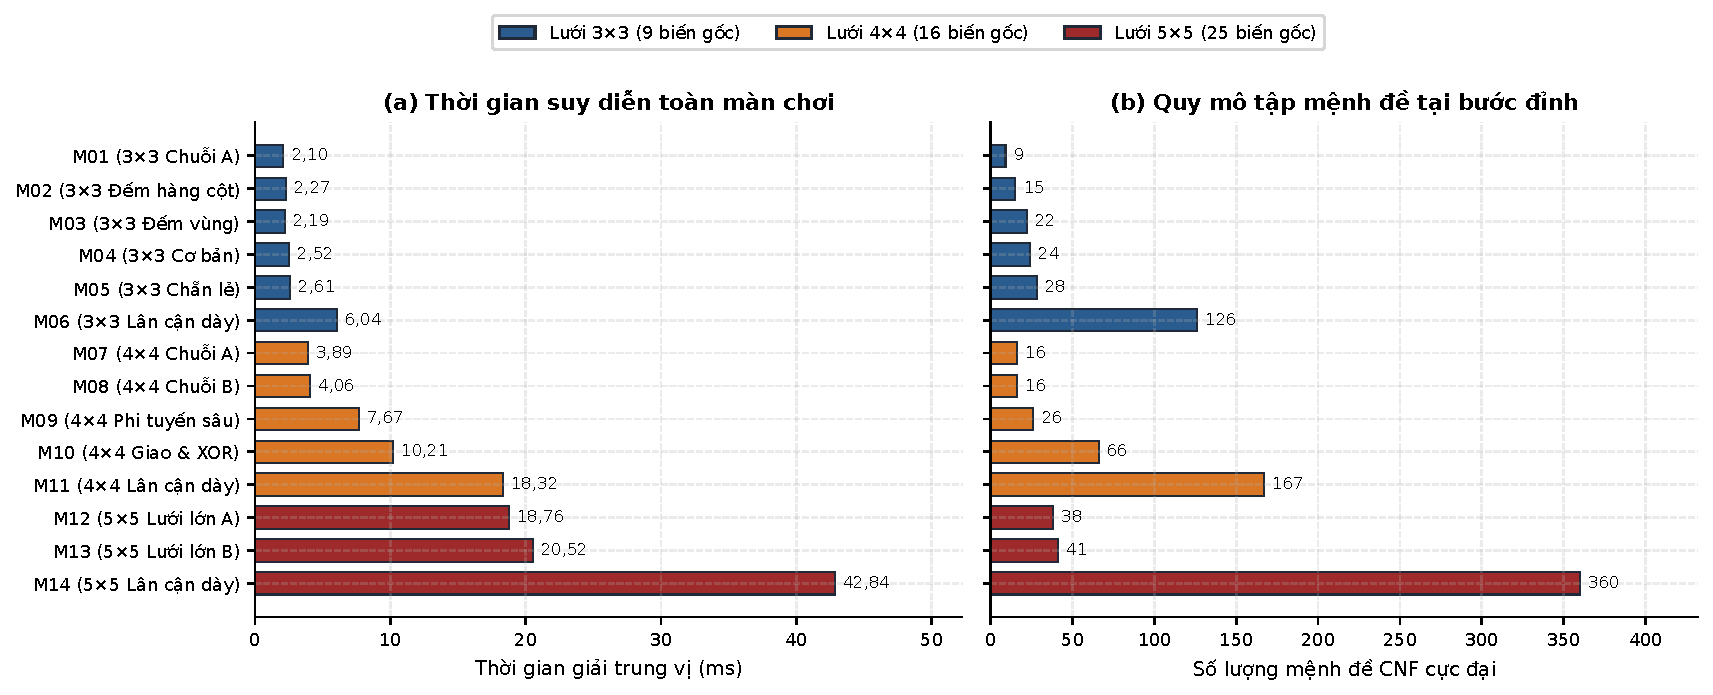
\includegraphics[width=0.98\textwidth]{images/charts/runtime_and_clauses.pdf}
    \caption{Đối sánh thời gian suy diễn trung vị (a) và số lượng mệnh đề CNF cực đại tại bước đỉnh (b) trên 14 màn chơi từ $3 \times 3$ đến $5 \times 5$}
    \label{fig:runtime_and_clauses}
\end{figure}

Đi sâu phân tích mối tương quan giữa cấu trúc mệnh đề và hành vi tìm kiếm bên trong bộ giải DPLL, số liệu thực nghiệm làm nổi bật hiệu lực áp đảo của cơ chế lan truyền mệnh đề đơn vị trên lớp bài toán suy diễn không đoán mò. Cụ thể, trên mười hai trong tổng số mười bốn màn chơi, số phép rẽ nhánh quyết định bằng không tuyệt đối, và trên toàn bộ mười bốn màn chơi không hề xuất hiện bất kỳ thao tác quay lui nào ($\text{Quay lui} = 0$). Hiện tượng này bắt nguồn từ bản chất toán học của câu đố: khi một ô thực sự bị ép buộc bởi các lời khai đang mở, việc tiêm giả định trái dấu vào cơ sở tri thức sẽ kích hoạt một thác rút gọn liên hoàn trên các mệnh đề bậc hai và bậc ba, làm bộc lộ mệnh đề rỗng ngay ở tầng gốc của thủ tục lan truyền mà không cần mở cây tìm kiếm. Ngay cả tại hai màn lân cận phức tạp $\text{M11}$ ($2$ quyết định) và $\text{M14}$ ($1$ quyết định), các phép chọn biến tự do này chỉ diễn ra ở nhánh kiểm tra khả thỏa của một ô chưa đủ dữ kiện để hoàn thiện nhanh mô hình chứng nhân và thành công ngay ở nhánh thử đầu tiên.

Bên cạnh đó, biểu đồ phân tán hai chiều tại Hình \ref{fig:regimes_scatter} cho thấy thời gian thực thi tổng thể không tăng đơn điệu thuần túy theo kích thước bàn cờ, mà phân tách rõ rệt thành \textbf{hai chế độ chi phí tính toán đối lập nhau}. Ở chế độ thứ nhất bị chi phối bởi khối lượng truy vấn và lan truyền (điển hình là hai màn $\text{M12}$ và $\text{M13}$ trên lưới $5 \times 5$), tập mệnh đề rất gọn nhẹ ($38$ đến $41$ mệnh đề), song các điểm mở khóa suy diễn lại thường nằm sâu ở các hàng cuối bàn cờ; do tác tử luôn quét tuần tự từ góc trái trên xuống dưới, mỗi bước phải thẩm định qua nhiều ô chưa xác định trước khi chạm tới ô ép buộc, đẩy tổng số lượt gọi SAT lên $228$ lần cùng $2.563$ phép lan truyền đơn vị và tiêu tốn $20{,}52\text{ ms}$. Trái ngược hoàn toàn, ở chế độ thứ hai bị chi phối bởi mật độ mệnh đề tổ hợp (điển hình là $\text{M06}$, $\text{M11}$ và đặc biệt là $\text{M14}$), tác tử chỉ cần $67$ truy vấn SAT và $870$ phép lan truyền (ít hơn gần ba lần so với $\text{M13}$), nhưng thời gian chạy lại tăng gấp đôi lên mức đỉnh $42{,}84\text{ ms}$. Nguyên nhân sâu xa nằm ở chỗ một lời khai đếm chính xác $4$ tội phạm trên vùng tám ô lân cận bên trong lưới đã sinh tới $\binom{8}{5} + \binom{8}{4} = 126$ mệnh đề, đẩy quy mô tập mệnh đề của $\text{M14}$ lên $360$ mệnh đề và làm gia tăng đáng kể chi phí duyệt danh sách mệnh đề bên trong từng chu kỳ lan truyền đơn vị.

\begin{figure}[H]
    \centering
    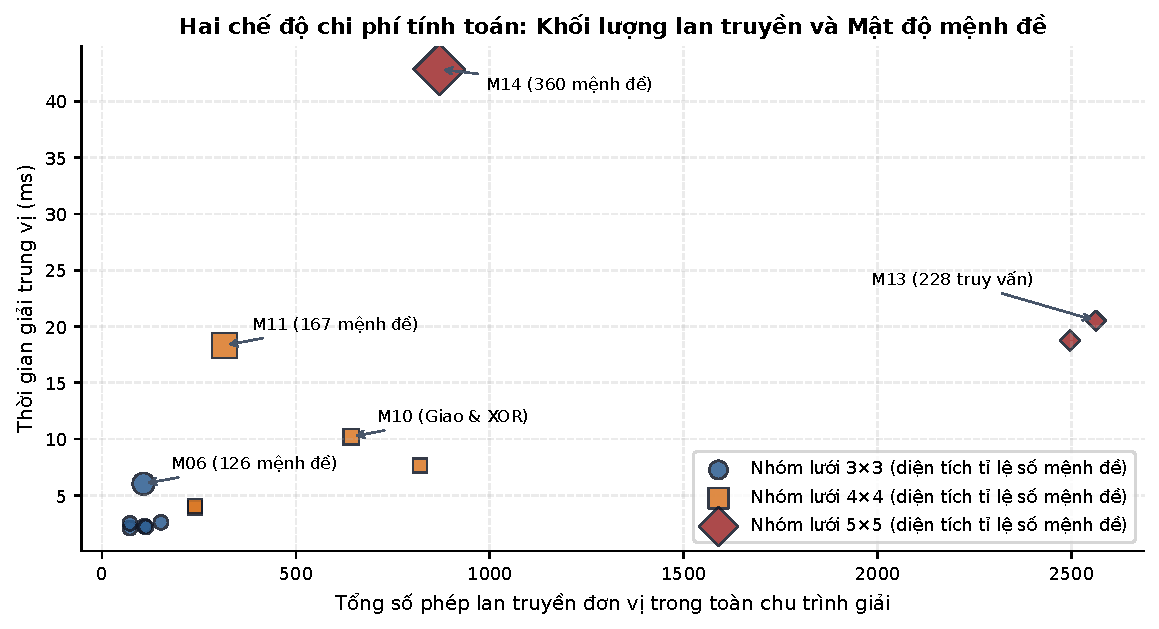
\includegraphics[width=0.78\textwidth]{images/charts/queries_vs_propagations.pdf}
    \caption{Sự phân hóa rõ nét giữa chế độ chi phối bởi mật độ mệnh đề tổ hợp (nhóm diện tích điểm lớn $\text{M06}, \text{M11}, \text{M14}$) và chế độ chi phối bởi khối lượng truy vấn ($\text{M12}, \text{M13}$)}
    \label{fig:regimes_scatter}
\end{figure}

\subsection{Đánh giá bóc tách bộ nhớ đệm}
\label{subsec:exp_ablation}
Nhằm kiểm chứng thực nghiệm giá trị của Mệnh đề 2 (Mục \ref{subsec:witness_cache}), nhóm thực hiện thí nghiệm bóc tách trên toàn bộ mười bốn màn chơi bằng cách đặt tác tử hoạt động ở hai chế độ đối chứng: tắt hoàn toàn bộ nhớ đệm mô hình chứng nhân (luôn thực hiện trọn vẹn cặp truy vấn giả định ngược cho từng ô) và bật bộ nhớ đệm mô hình chứng nhân theo từng bước. Hình \ref{fig:witness_ablation} và Bảng \ref{tab:ablation_summary} cho thấy việc tái sử dụng các mô hình thỏa mãn đã giúp cắt giảm tổng số lượt gọi DPLL trên toàn tập dữ liệu từ $930$ lượt xuống còn $863$ lượt (tiết kiệm $67$ lượt giải SAT, tương đương mức giảm $7{,}20\%$), đồng thời kéo giảm tổng số phép lan truyền đơn vị từ $9.493$ phép xuống $8.813$ phép (giảm $7{,}16\%$) mà vẫn giữ nguyên tuyệt đối thứ tự các bước suy diễn.

\begin{figure}[H]
    \centering
    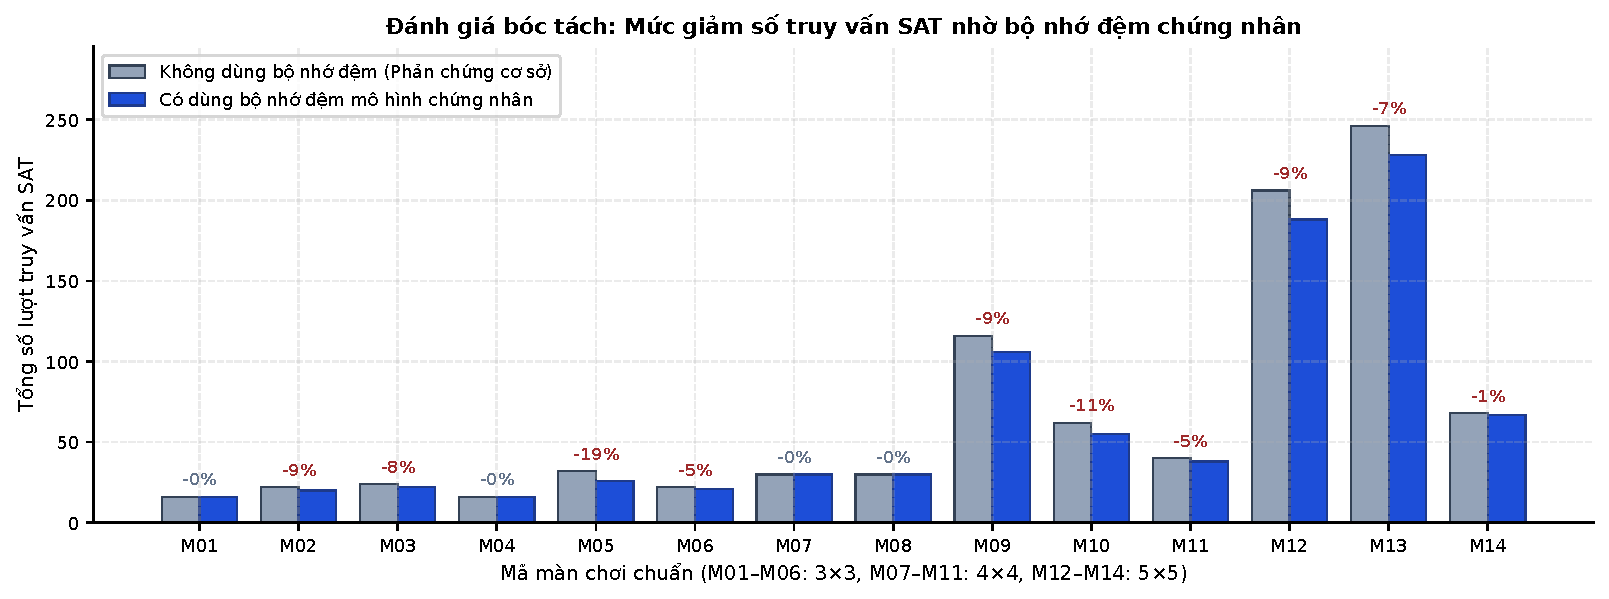
\includegraphics[width=0.96\textwidth]{images/charts/witness_cache_ablation.pdf}
    \caption{Kết quả thí nghiệm bóc tách số lượng truy vấn SAT khi tắt và bật bộ nhớ đệm mô hình chứng nhân trên 14 màn chơi}
    \label{fig:witness_ablation}
\end{figure}

\begin{table}[H]
\centering
\caption{Đối sánh định lượng hiệu quả của bộ nhớ đệm mô hình chứng nhân trên các màn chơi đại diện}
\label{tab:ablation_summary}
\resizebox{\textwidth}{!}{%
\begin{tabular}{l l c r r c r r c}
\toprule
\textbf{Mã} & \textbf{Đặc trưng tô-pô suy diễn} & \textbf{Lưới} & \textbf{Truy vấn (Tắt)} & \textbf{Truy vấn (Bật)} & \textbf{Tỷ lệ giảm} & \textbf{Lan truyền (Tắt)} & \textbf{Lan truyền (Bật)} & \textbf{Tỷ lệ giảm} \\
\midrule
M04 & Chuỗi thuận thứ tự quét hàng & $3\times3$ & 16  & 16  & $0{,}00\%$            & 72    & 72    & $0{,}00\%$ \\
M05 & Chẵn lẻ vùng nhảy cóc        & $3\times3$ & 32  & 26  & \textbf{$-18{,}75\%$} & 182   & 152   & \textbf{$-16{,}48\%$} \\
M07 & Chuỗi thuận thứ tự quét hàng & $4\times4$ & 30  & 30  & $0{,}00\%$            & 240   & 240   & $0{,}00\%$ \\
M09 & Suy diễn phi tuyến cuối bảng & $4\times4$ & 116 & 106 & $-8{,}62\%$           & 896   & 820   & $-8{,}48\%$ \\
M10 & Giao vùng kết hợp chuỗi XOR  & $4\times4$ & 62  & 55  & \textbf{$-11{,}29\%$} & 725   & 643   & \textbf{$-11{,}31\%$} \\
M12 & Mạng lưới rộng phi tuyến     & $5\times5$ & 206 & 188 & $-8{,}74\%$           & 2.735 & 2.496 & $-8{,}74\%$ \\
M13 & Mạng lưới rộng chuyên sâu    & $5\times5$ & 246 & 228 & $-7{,}32\%$           & 2.781 & 2.563 & $-7{,}84\%$ \\
\midrule
\multicolumn{2}{l}{\textbf{Tổng cộng toàn bộ 14 màn chơi}} & -- & \textbf{930} & \textbf{863} & \textbf{$-7{,}20\%$} & \textbf{9.493} & \textbf{8.813} & \textbf{$-7{,}16\%$} \\
\bottomrule
\end{tabular}%
}
\end{table}

Sự phân hóa tỷ lệ tiết kiệm giữa các màn chơi trong Bảng \ref{tab:ablation_summary} được giải thích rất nhất quán dưới góc độ tô-pô thứ tự suy diễn. Ở những màn chơi có lộ trình mở khóa thuận theo chiều quét ưu tiên hàng như $\text{M01}$, $\text{M04}$, $\text{M07}$ và $\text{M08}$, tại mọi bước lập luận, ngay ô chưa mở đầu tiên mà tác tử xét tới đã chính là ô bị ép buộc chân trị ($15\text{ bước} \times 2\text{ truy vấn} = 30\text{ truy vấn}$), do đó vòng lặp kết thúc bước ngay lập tức trước khi có bất kỳ ô chưa xác định nào được lưu chứng nhân ($0\%$ khác biệt). Ngược lại, trên những màn chơi có mạch suy diễn phi tuyến đòi hỏi nhảy vọt giữa các hàng cột xa nhau như $\text{M05}$, $\text{M09}$, $\text{M10}$, $\text{M12}$ và $\text{M13}$, ngay khi tác tử đi qua ô chưa xác định đầu tiên, hai mô hình thỏa mãn thu được sẽ phủ kín giá trị chân trị cho phần lớn các biến liên đới trên bàn cờ, giúp miễn trừ tức khắc một nửa số lượt gọi DPLL cho các ô tiếp theo và đem lại mức tiết kiệm lên tới $18{,}75\%$ trên màn $\text{M05}$ và $11{,}29\%$ trên màn $\text{M10}$.

\subsection{Phân tích độ mở rộng mệnh đề}
\label{subsec:exp_scaling}
Tiếp nối phân tích hiệu năng thời gian, Hình \ref{fig:encoding_scaling} khảo sát quy luật tăng trưởng số lượng mệnh đề CNF sinh ra khi kích thước vùng tác động $m = |R|$ mở rộng từ $2$ ô lên $16$ ô giữa ba chiến lược biên dịch: mã hóa chẵn lẻ trực tiếp từ bảng chân trị ($2^{m-1}$ mệnh đề, không biến phụ), mã hóa đếm lực lượng tổ hợp tại ngưỡng cân bằng $\lfloor m/2 \rfloor$ ($\binom{m}{\lfloor m/2 \rfloor + 1} + \binom{m}{\lceil m/2 \rceil + 1}$ mệnh đề, không biến phụ), và mã hóa chuỗi cổng tuyển loại trừ sử dụng $m - 2$ biến phụ Tseitin ($4m - 6$ mệnh đề). Ở phạm vi vùng rất hẹp $m \in \{3, 4\}$, cách mã hóa không biến phụ tỏ ra nhỉnh hơn đôi chút nhờ chỉ sinh từ $4$ đến $8$ mệnh đề ngắn. Thế nhưng ngay khi vượt qua ngưỡng $m \ge 6$, cả hai phương pháp không biến phụ đều bùng nổ theo tiệm cận hàm mũ Stirling $\binom{m}{m/2} \sim 2^m / \sqrt{\pi m / 2}$, trong khi đường biểu diễn của chuỗi cổng XOR biến phụ vẫn giữ độ dốc tuyến tính phẳng lặng. Tại mốc $m = 16$ (tương đương một lời khai bao trùm toàn bộ bàn cờ $4 \times 4$), bảng chân trị trực tiếp phát sinh tới $32.768$ mệnh đề và phép đếm tổ hợp phát sinh $22.880$ mệnh đề, trong khi mạch dây chuyền biến phụ chỉ cần vỏn vẹn $58$ mệnh đề bậc ba --- thu gọn dung lượng cơ sở tri thức tới $565$ lần.

\begin{figure}[H]
    \centering
    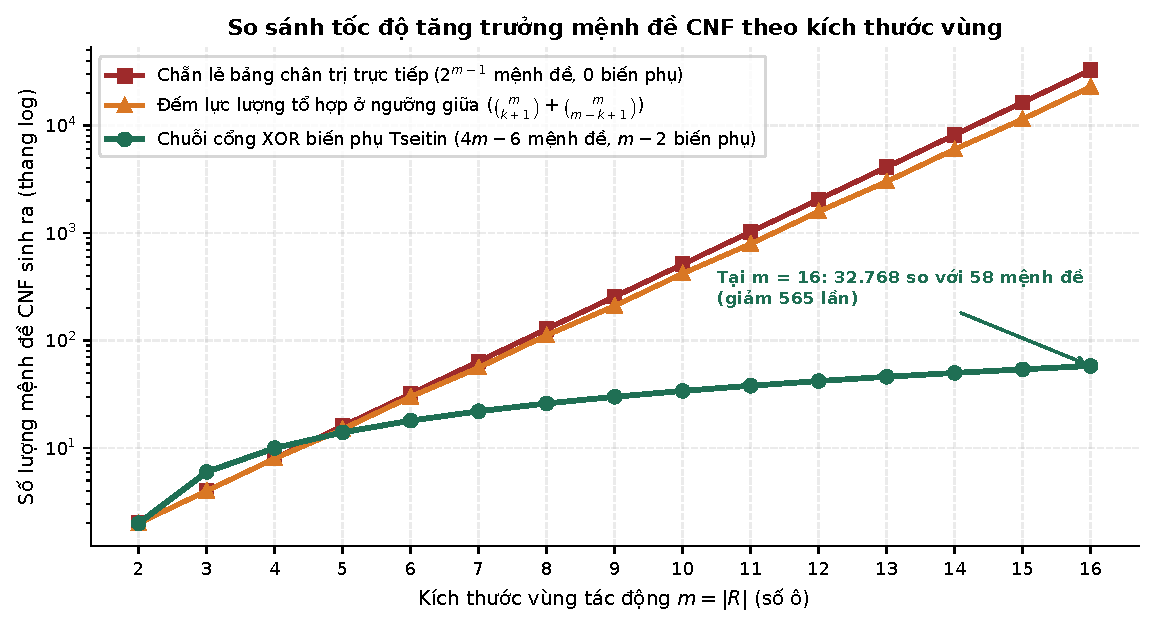
\includegraphics[width=0.78\textwidth]{images/charts/encoding_clause_scaling.pdf}
    \caption{Đối sánh tốc độ tăng trưởng mệnh đề CNF (trục tung logarit) giữa phương pháp hàm mũ/tổ hợp không biến phụ và chuỗi cổng XOR biến phụ tuyến tính}
    \label{fig:encoding_scaling}
\end{figure}

\subsection{Kịch bản biên và giới hạn hệ thống}
\label{subsec:exp_limitations}
Một báo cáo thực nghiệm khách quan không chỉ dừng lại ở các trường hợp thành công thuận lợi mà cần mổ xẻ thẳng thắn cách hệ thống phản ứng trước dữ liệu suy biến cũng như những điểm nghẽn kiến trúc khi đẩy bài toán tới cực hạn. Để phục vụ mục đích này, nhóm thiết kế bốn kịch bản đối kháng có kiểm soát (ký hiệu từ $\text{K01}$ đến $\text{K04}$) và ghi nhận kết quả thực thi thực tế trong Bảng \ref{tab:failure_stress}. Ở kịch bản thiếu dữ kiện $\text{K01}$ (chỉ cho biết hàng đầu tiên có đúng một tội phạm trong khi hai ô $\text{B1}$ và $\text{C1}$ hoàn toàn đối xứng nhau), quy trình kiểm định nghiệm duy nhất phát hiện ngay sự tồn tại của nghiệm thứ hai chỉ sau hai lượt giải, đồng thời chu trình giải tự động dừng lại an toàn ngay ở bước đầu tiên sau $14$ truy vấn kiểm tra mà không hề mạo hiểm đoán mò. Tương tự ở kịch bản dữ liệu hỏng $\text{K02}$ (một lời khai khẳng định $\text{B1}$ là tội phạm nhưng lời khai khác lại cấm toàn bộ hàng đầu tiên có tội phạm), tác tử lập tức phát hiện cơ sở tri thức vô nghiệm chỉ trong $0{,}11\text{ ms}$ và ngắt chu trình trước khi làm sai lệch trạng thái bàn cờ.

\begin{table}[H]
\centering
\caption{Kết quả kiểm thử các kịch bản suy biến có kiểm soát và bài toán vô nghiệm áp lực cao}
\label{tab:failure_stress}
\scriptsize
\setlength{\tabcolsep}{4.5pt}
\begin{tabularx}{\textwidth}{l >{\raggedright\arraybackslash}X r r r r r c}
\toprule
\textbf{Mã} & \textbf{Cấu trúc ràng buộc đối kháng} & \textbf{Mệnh đề} & \textbf{Nhánh} & \textbf{Lan truyền} & \textbf{Quay lui} & \textbf{Thời gian (ms)} & \textbf{Kết cục xử lý} \\
\midrule
K01 & Màn $3\times3$ khuyết thiếu dữ kiện khiến hai ô đối xứng hoàn toàn & 6  & 0     & 28    & 0     & 0,84  & Dừng an toàn (Đa nghiệm) \\
K02 & Màn $3\times3$ chứa hai lời khai trực tiếp phủ định lẫn nhau       & 5  & 0     & 2     & 0     & 0,11  & Ngắt an toàn (Mâu thuẫn) \\
K03 & Lưới $4\times4$ vô nghiệm đếm: 4 hàng có đúng 2 tội phạm nhưng 4 cột có tối đa 1 & 56 & 10    & 71    & 10    & 0,65  & Bác bỏ thành công \\
K04 & Lưới $4\times4$ vô nghiệm chẵn lẻ: 4 hàng tổng chẵn nhưng 3 cột tổng lẻ và 1 cột chẵn & 80 & \textbf{1.022} & \textbf{5.220} & \textbf{1.022} & \textbf{87,24} & Bác bỏ thành công \\
\bottomrule
\end{tabularx}
\end{table}

Đáng chú ý hơn cả là sự tương phản sâu sắc giữa hai bài toán vô nghiệm toàn cục trên lưới $4 \times 4$ ($\text{K03}$ và $\text{K04}$), qua đó phơi bày ba giới hạn kỹ thuật trung thực của hệ thống hiện tại. Giới hạn thứ nhất nằm ở \textbf{điểm mù phân giải của giải thuật DPLL thuần túy trước hệ phương trình tuyến tính trên trường hữu hạn $\mathbb{F}_2$} \cite{tseitin1983complexity,urquhart1987hard}: trong khi mâu thuẫn tổng lực lượng ở $\text{K03}$ ($8 \ne 4$) được DPLL bác bỏ dễ dàng chỉ sau $10$ nhánh quay lui ($0{,}65\text{ ms}$), thì mâu thuẫn chẵn lẻ toàn cục ở $\text{K04}$ (tổng bốn hàng chẵn bằng $0 \pmod 2$ đối chọi với tổng ba cột lẻ cộng một cột chẵn bằng $1 \pmod 2$) lại buộc bộ giải phải duyệt sâu tới $1.022$ quyết định rẽ nhánh, $5.220$ phép lan truyền và $1.022$ lần quay lui trong $87{,}24\text{ ms}$. Nguyên nhân là mỗi mệnh đề bậc ba của cổng XOR chỉ có thể kích hoạt lan truyền đơn vị khi đã biết trước hai trong ba biến; do không tích hợp phép khử Gauss--Jordan chuyên biệt \cite{soos2009extending}, DPLL buộc phải rẽ nhánh mũ trên cây tìm kiếm mới phát hiện ra tính vô nghiệm toàn cục. Giới hạn thứ hai là phép biên dịch đếm lực lượng hiện chưa sử dụng biến phụ bộ đếm tuần tự \cite{sinz2005towards}; dù rất nhanh trên các vùng $\le 8$ ô, nếu áp dụng cho một lời khai đếm $12$ tội phạm trên toàn mặt bàn $5 \times 5$ ($m = 25$), tổ hợp $\binom{25}{13} + \binom{25}{14}$ sẽ vượt ngưỡng chín triệu mệnh đề và gây tràn bộ nhớ. Cuối cùng, giới hạn thứ ba đến từ việc bộ giải được cài đặt trên ngôn ngữ thông dịch bậc cao với thao tác quét tuần tự danh sách mệnh đề và sao chép bảng gán khi rẽ nhánh thay vì cấu trúc hai con trỏ theo dõi (\textit{two-watched literals}) và học mệnh đề xung đột (\textit{CDCL}) \cite{silva1999grasp,moskewicz2001chaff}, khiến tốc độ xử lý sẽ suy giảm nếu mở rộng lên quy mô lưới lớn cỡ $10 \times 10$.
